

\chapter{Surface plasmon polaritons} 

\section{Introduction}

The interaction of light with metals has long proven to be a reliable path to striking optical effects.  The Lycurgus cup is an example of a 4th century plasmonic device; a glass Roman goblet which uses colloidal gold and silver nano-particles to achieve a dull green surface reflection, but glows blood red when illuminated from the inside \cite{Barber1990}.  Resonant interaction between light and the electrons in these suspended metallic nano-particles provide the mechanism for this vivid dichic effect, the same effect found in the majority of stained glass windows. 

Surface plasmon polaritons are electromagnetic surface waves coupled strongly to the longitudinal oscillations of the free electron plasma at the interface between a dielectric and a metal. 

\section{Surface Polaritons on planar surfaces}


Surface plasmon polaritons can be categorized as a member of a larger family of surface waves, broadly named `surface polaritons'. Surface polaritons are electromagnetic surface waves coupled strongly to an elementary excitation and bound evanescently to the interface between two mediums. When a photon couples to the longitudinal oscillations of the free-electron plasma on metal surfaces, the resulting surface polariton is called a \textit{surface plasmon polariton}. Surface polaritons also couple with surface lattice vibrations (\textit{surface phonon polaritons}), surface electron-hole pairs in semiconductors (\textit{surface exciton polaritons}) and collective excitations of surface electron spin (\textit{surface magnon polaritons}). More recently, the manufacture of resonant sub-wavelength structures, or `metamaterials', has allowed the design of surfaces with tailored resonances other than such elementary excitations, which may couple strongly to photons and produce surface polaritons. The resulting surface polaritons are often referred to as a `spoof' surface plasmon polaritons.\footnote{although the inclusion of `plasmon' is not strictly correct as the photon is not coupled to the free electron plasma oscillations but more usually a sub-wavelength cavity resonance.}
Solving Maxwell's equations for a evanescently bound electromagnetic wave at an interface leads to the same relationship between energy and momentum for all surface polaritons. The coupling of light to the surface excitations is expressed in terms of the frequency dependant dielectric and magnetic functions which are frequency dependant and complex in general.

Fano \cite{Fano1941} derived the dispersion for a trapped surface wave by first considering light propagating in a glass plate of finite thickness, bounded by semi-infinite vacuum and metal half-spaces.  In a simple waveguide such as this, total internal reflections prevent the propagating light from escaping into the bounding medium. The necessary continuity of electric field across a boundary for light undergoing total internal reflection also requires non-propagating 'evanescent' waves extending into the bounding media, which do not  transfer any power. The question posed by Fano was then `Is there left any proper value when the thickness vanishes?'. As the thickness of the glass plate tends to zero, there is indeed still a valid solution to Maxwell's equations for a wave travelling along the surface, evanescently bound in the normal direction; a surface polariton. In these terms, a surface polariton can be thought of as the lowest-order waveguide mode.

Generally, the dispersion relation for all surface polaritions are identical, with the coupling of the electromagnetic surface wave to the surface excitations being expressed in the different functional forms of the dielectric and magnetic tensors of the bounding media.  

The dispersion of the surface polarition considered in this thesis, the surface plasmon polarition on a metal/dielectric interface, allows us to simplify the problem to that of isotropic, non-magnetic media. The derivation of this relationship\cite{Raether1988} is presented below, and is also valid for other surface polaritions in isotropic non-magnetic media, such as surface phonon polaritions.

\begin{figure}[h]
\begin{center}
\begin{pspicture}[](8,5) %start optics diagram (8x5) grid
	\pnode(4,2){C} %labeled nodes are the positions in the (8x5) grid
	\pnode(0.5,5){i} %labeled nodes are the positions in the (8x5) grid
	\pnode(7.5,5){r} %labeled nodes are the positions in the (8x5) grid
	\pnode(8,0.5){t}
	
	\addtopsstyle{ExtendedMirror}{hatchcolor=lightgray}
	\polarization[labeloffset=0.6](i)(C){$\mathbf{E}_0$}
	\mirror[mirrorwidth=8,mirrortype=extended,mirrordepth=2](i)(C)(r)
	\polarization[labeloffset=0.6](C)(r){$\mathbf{E}_1$}
	\polarization[labeloffset=0.6](C)(t){$\mathbf{E}_2$}
	\psline[linestyle=dashed](4,5)(4,0)
	\drawbeam[beam,ArrowInside=->,arrowscale=1](i){1}{2}{3}{(r)}
	\drawbeam[beam,ArrowInside=->,arrowscale=1](C){4}{(t)}
	%\psarcAB(C)(4,3)(3,2)
	\psline{->}(0.5,0.5)(0.5,1.25)
	\psline{->}(0.5,0.5)(1.25,0.5)
	\rput(1.5,0.5){$\mathbf{\hat{x}}$}
	\rput(0.5,1.5){$\mathbf{\hat{z}}$}
	\rput(7.5,1.5){$\varepsilon_2$}
	\rput(7.5,2.5){$\varepsilon_1$}
	\rput(1.55,4.65){\green $\mathbf{k}_0$}
	\rput(6.45,4.65){\green $\mathbf{k}_1$}
	\rput(6.75,0.55){\green $\mathbf{k}_2$}
\end{pspicture}
\end{center}
\caption{\label{fig:planar-coords}A schematic representation of propagating electromagnetic fields at an interface between two materials. The green rays illustrate the direction of the waves, which are coincident with the wavevectors, \color{green}$\mathbf{k}$\color{black}. The electric field is polarised in the $Oxz$ plane, represented by black arrows. The optical response of the two media are characterised by their permativities, $\varepsilon_1$ and $\varepsilon_2$. The $\mathbf{\hat{y}}$-direction is out of the page and the position $z=0$ is at the interface. }
\end{figure}

A schematic diagram of the system is shown in figure \ref{fig:planar-coords}. Light illuminates a planar surface between two media of permittivities $\varepsilon_1$ and $\varepsilon_2$ in the $Oxz$ plane, which we define to be the plane of incidence. The wavevector of the light in the $m^{th}$ medium is $\mathbf{k}_m = k_{x_m}\mathbf{\hat{x}}+k_{z_m}\mathbf{\hat{z}} \equiv [k_{x_m},0,k_{z_m}]$, with no component in the $\mathbf{\hat{y}}$-direction (out of the page). The light is then reflected back into medium 1 and refracted into medium 2.  For light polarised with the electric field parallel to the plane of incidence (Transverse Magnetic, or TM polarised) the plane waves can be described as,
\begin{align*}
\mathbf{E}_m&=[E_{x_m},0,E_{z_m}]\:e^{i(\mathbf{k}_m\cdot \mathbf{x}+\mathbf{k}_m\cdot\mathbf{z})}\:e^{-i\omega t}\\
\mathbf{H}_m&=[0,H_{y_m},0]\:e^{i(\mathbf{k}_m\cdot \mathbf{x}+\mathbf{k}_m\cdot\mathbf{z})}\:e^{-i\omega t}
\end{align*}
where $\omega$ is the angular frequency of the light, $t$ is time and $m$ is a subscript indicating in which medium the field is propagating. $H_{y}$ is the component of magnetic field in the $\mathbf{\hat{y}}$-direction and $E_{x,z}$ is the component of electric field in the $\mathbf{\hat{x}}$ and  $\mathbf{\hat{z}}$ directions, respectively. 
Since the surface polarition is a trapped surface wave, we may arbitrarily set either the incident or reflected wave to zero. Setting, in this case, $\mathbf{E}_0$ to zero, we are left with two sets of fields (electric and magnetic) for the half-spaces above and below the interface,
\begin{align}
z>0\;\begin{cases}\;\mathbf{E}_1&=\;[E_{x_1},0,E_{z_1}]\:e^{i(k_{x_1}x+k_{z_1}z)}\:e^{-i\omega t}\\
\;\mathbf{H}_1&=\;[0,H_{y_1},0]\:e^{i(k_{x_1}x+k_{z_1}z)}\:e^{-i\omega t}
\end{cases}\label{eq:planewaveset1}\\
z<0\;\begin{cases}\;\mathbf{E}_2&=\;[E_{x_2},0,E_{z_2}]\:e^{i(k_{x_2}x-k_{z_2}z)}\:e^{-i\omega t}\\
\;\mathbf{H}_2&=\;[0,H_{y_2},0]\:e^{i(k_{x_2}x-k_{z_2}z)}\:e^{-i\omega t}
\end{cases}\label{eq:planewaveset2}
\end{align}
We may combine the equations for electric and magnetic field in the two half-spaces using Amp\`ere's law,
\begin{equation*}
\mathbf{\nabla}\times\mathbf{H}_m=\varepsilon_m\:\frac{\partial\mathbf{E}_m}{\partial t}
\end{equation*}
where $\varepsilon_m$ is the permittivity in medium $m$. The relationships between the tangential electric and transverse magnetic fields in each material are then,
\begin{align}
%k_{z_1}H_{y_1}&=+\frac{\omega}{c}\varepsilon_1E_{x_1}\label{eq:tangentE-transverE1}\\
k_{z_1}H_{y_1}&=+\omega\varepsilon_1E_{x_1}\label{eq:tangentE-transverE1}\\
%k_{z_2}H_{y_2}&=-\frac{\omega}{c}\varepsilon_2E_{x_2}\label{eq:tangentE-transverE2}
k_{z_2}H_{y_2}&=-\omega\varepsilon_2E_{x_2}\label{eq:tangentE-transverE2}
\end{align}
Having obtained expressions for the electromagnetic fields in both media, we must now consider the continuity of these fields over the boundary. At the interface the boundary conditions for the electromagnetic waves are expressed as,
\begin{align}
E_{x_1}&=E_{x_2}\label{eq:electric-field-continuous}\\
H_{y_1}&=H_{y_2}\label{eq:magnetic-field-continuous}\\
\varepsilon_1E_{z_1}&=\varepsilon_2E_{z_2}\label{eq:d-continuous}
\end{align}
These are the conditions that tangential electric fields, transverse magnetic fields and the normal component of the electric displacement vector ($D_{z_m}=\varepsilon_m E_{z_m}$) must be continuous across the boundary at $z=0$. The continuity of the tangential electric field (equation \ref{eq:electric-field-continuous}) allows us to combine equations \ref{eq:tangentE-transverE1} and \ref{eq:tangentE-transverE2},
\begin{equation*}
\frac{k_{z_1}}{\varepsilon_1}H_{y_1}+\frac{k_{z_2}}{\varepsilon_2}H_{y_2}=0
\end{equation*}
and continuity of transverse magnetic field (equation \ref{eq:magnetic-field-continuous}) then yields\footnote{At this point, we also employ some mathematical sleight of hand to substitute the permittivity, $\varepsilon_m$, for the relative permittivity ($\varepsilon_m/\varepsilon_0$) by cancelling the common factor of $\varepsilon_0$ in $\varepsilon_1$ and $\varepsilon_2$. For clarity we redefine $\varepsilon_m$ as the \textit{relative} permittivity for the remainder of this thesis.}
\begin{align}
\frac{k_{z_1}}{\varepsilon_1}+\frac{k_{z_2}}{\varepsilon_2}=0\label{eq:relation-of-kz1-kz2}
\end{align}
Finally, to obtain a relationship in terms of the momentum of the surface wave in the $\mathbf{\hat{x}}$-direction ($k_x$), we consider the conservation of momentum in both regions.  Conservation of tangential momentum  requires that $k_{x_1}=k_{x_2}=k_x$ and so the expression for total conserved momentum is,
\begin{equation}
k_x^2+k_{z_m}^2=\varepsilon_m\left(\frac{\omega}{c}\right)^2\label{eq:momentum-conservation}
\end{equation}
Obtaining expressions for $k_{z_1}$ and $k_{z_2}$ using this conservation of momentum expression and combining them with equation \ref{eq:relation-of-kz1-kz2}, we find the dispersion relation for the surface polariton,
\begin{equation}
k_x=\frac{\omega}{c}\sqrt{\frac{\varepsilon_1\varepsilon_2}{\varepsilon_1+\varepsilon_2}}\label{eq:dispersion}
\end{equation}
This equation relates the angular frequency of the field, $\omega$ to the wavevector along the surface, $k_x$. The energy and momentum of the surface mode is related to these quantities respectively by a factor of the reduced Planks constant, $\hbar$. Because of this, it is also often referred to as the energy-momentum relation.  

The final observation to be made in regards to the surface polarition dispersion is the set of $\varepsilon_1$ and $\varepsilon_2$ values which can support a bound surface wave. The continuity of tangential electric displacement was mentioned briefly in equation \ref{eq:d-continuous}, and we shall re-print it here.
\begin{equation*}
\varepsilon_1E_{z_1}=\varepsilon_2E_{z_2}
\end{equation*}
This boundary condition states that the tangential electric displacement must remain continuous across the interface. However, from the plane wave equation sets (equations \ref{eq:planewaveset1}--\ref{eq:planewaveset2}) it is apparent that $E_{z_1}$ is always $180^{\circ}$ out-of-phase with $E_{z_2}$. $E_{z_1}$ will always be of opposite sign to $E_{z_2}$. To satisfy the boundary condition, and so support surface polaritons on such a surface, the permativities $\varepsilon_1$ and $\varepsilon_2$ must also be of opposite signs. 

\section{Dispersion of Surface Plasmon Polaritons on planar surfaces}

The optical response of a metal is characterized by the metal's frequency dependant permittivity, also called the `dielectric function' of the material. This optical response function is dominated by two characteristics of metal materials; the fact that conduction electrons are free to move within the bulk of the material, and the presence of inter-band transitions of the valence electrons in the atomic orbitals. In the visible region, conduction electrons behaviour is ballistic, oscillating and interacting with light many times before scattering due to the crystal or other electrons. The inter-band transitions for a noble metal such as silver occur at the edges of the visible spectrum and so the dominant effect in the appearance of silver is due mostly to the strong interaction of the free conduction electrons with optical fields. At the surface of the metal, electromagnetic fields coupled to longitudinal oscillations of this free-electron plasma form together a surface polariton, the surface plasmon polarition.

The dispersion of a surface plasmon polarition takes the same mathematical form as equation \ref{eq:dispersion} with one dielectric function representing the frequency dependant metal, $\varepsilon_2(\omega)$, and the other representing a bounding non-conducting crystal with a dielectric constant, $\varepsilon_1,$
\begin{equation}
k_x=\frac{\omega}{c}\sqrt{\frac{\varepsilon_1\varepsilon_2(\omega)}{\varepsilon_1+\varepsilon_2(\omega)}}\label{eq:spp-dispersion}
\end{equation}

A useful approximation for the metal dielectric function was presented by Drude. Drude considered free electrons travelling in a classical manner, scattering from the ionic lattice with a characteristic average scattering rate. Electron-electron scattering is disregarded and the permativty is expressed as,
\begin{equation}
\varepsilon_2(\omega)=\varepsilon_\infty-\frac{\omega_p^2}{\omega^2+i\omega\gamma}\label{eq:drude}
\end{equation}
Where $\omega$ is the angular frequency of the light, $\gamma$ is the average rate of collisions of the free conduction electrons with the lattice, and $\varepsilon_\infty$ is the response of the ionic lattice, which is frequency independent and for metals in the visible domain equals 1. The `plasma frequency' of the metal, $\omega_p$, is the limiting frequency ...

An example of the permittivity of silver using the Drude model is show in in figure \ref{fig:drude}. It shows that, for all visible regime wavelengths, that the real part of the silver permittivity is negative and there is a nono-zero imaginary component. This is generally true for a wide range of metals.
\begin{figure}
\begin{center}
% Created by tikzDevice version 0.6.2-92-0ad2792 on 2012-09-27 11:44:32
% !TEX encoding = UTF-8 Unicode
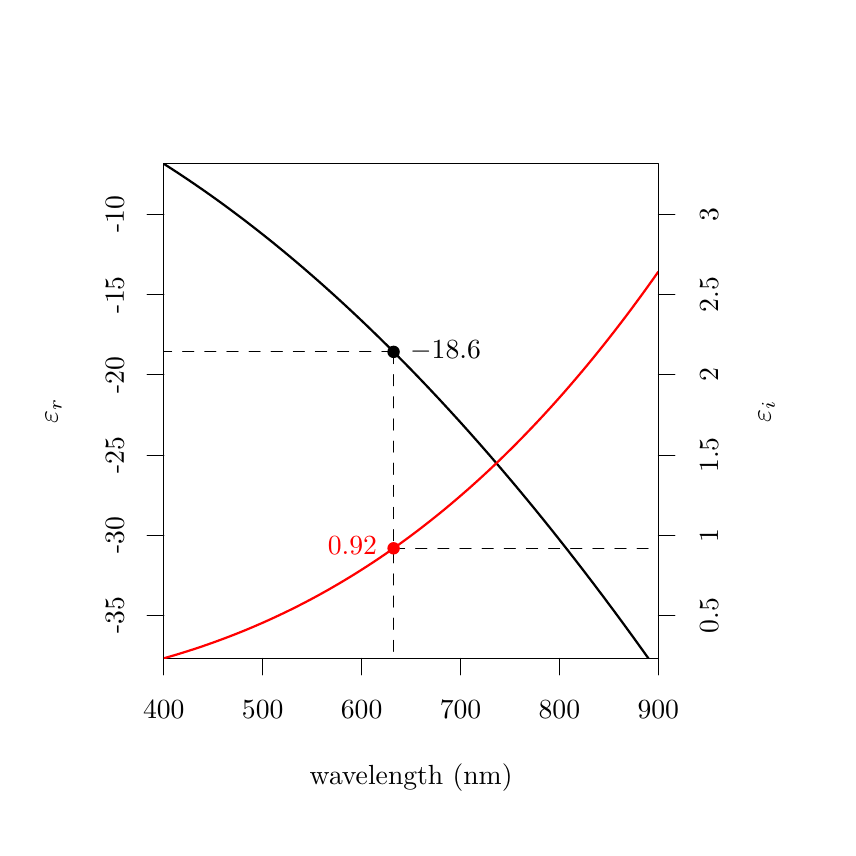
\begin{tikzpicture}[x=1pt,y=1pt]
\definecolor[named]{fillColor}{rgb}{1.00,1.00,1.00}
\path[use as bounding box,fill=fillColor,fill opacity=0.00] (0,0) rectangle (289.08,289.08);
\begin{scope}
\path[clip] (  0.00,  0.00) rectangle (289.08,289.08);
\definecolor[named]{drawColor}{rgb}{0.00,0.00,0.00}

\path[draw=drawColor,line width= 0.4pt,line join=round,line cap=round] ( 49.20, 61.20) -- (227.88, 61.20);

\path[draw=drawColor,line width= 0.4pt,line join=round,line cap=round] ( 49.20, 61.20) -- ( 49.20, 55.20);

\path[draw=drawColor,line width= 0.4pt,line join=round,line cap=round] ( 84.94, 61.20) -- ( 84.94, 55.20);

\path[draw=drawColor,line width= 0.4pt,line join=round,line cap=round] (120.67, 61.20) -- (120.67, 55.20);

\path[draw=drawColor,line width= 0.4pt,line join=round,line cap=round] (156.41, 61.20) -- (156.41, 55.20);

\path[draw=drawColor,line width= 0.4pt,line join=round,line cap=round] (192.14, 61.20) -- (192.14, 55.20);

\path[draw=drawColor,line width= 0.4pt,line join=round,line cap=round] (227.88, 61.20) -- (227.88, 55.20);

\node[text=drawColor,anchor=base,inner sep=0pt, outer sep=0pt, scale=  1.00] at ( 49.20, 39.60) {400};

\node[text=drawColor,anchor=base,inner sep=0pt, outer sep=0pt, scale=  1.00] at ( 84.94, 39.60) {500};

\node[text=drawColor,anchor=base,inner sep=0pt, outer sep=0pt, scale=  1.00] at (120.67, 39.60) {600};

\node[text=drawColor,anchor=base,inner sep=0pt, outer sep=0pt, scale=  1.00] at (156.41, 39.60) {700};

\node[text=drawColor,anchor=base,inner sep=0pt, outer sep=0pt, scale=  1.00] at (192.14, 39.60) {800};

\node[text=drawColor,anchor=base,inner sep=0pt, outer sep=0pt, scale=  1.00] at (227.88, 39.60) {900};

\path[draw=drawColor,line width= 0.4pt,line join=round,line cap=round] ( 49.20, 76.68) -- ( 49.20,221.56);

\path[draw=drawColor,line width= 0.4pt,line join=round,line cap=round] ( 49.20, 76.68) -- ( 43.20, 76.68);

\path[draw=drawColor,line width= 0.4pt,line join=round,line cap=round] ( 49.20,105.66) -- ( 43.20,105.66);

\path[draw=drawColor,line width= 0.4pt,line join=round,line cap=round] ( 49.20,134.63) -- ( 43.20,134.63);

\path[draw=drawColor,line width= 0.4pt,line join=round,line cap=round] ( 49.20,163.61) -- ( 43.20,163.61);

\path[draw=drawColor,line width= 0.4pt,line join=round,line cap=round] ( 49.20,192.59) -- ( 43.20,192.59);

\path[draw=drawColor,line width= 0.4pt,line join=round,line cap=round] ( 49.20,221.56) -- ( 43.20,221.56);

\node[text=drawColor,rotate= 90.00,anchor=base,inner sep=0pt, outer sep=0pt, scale=  1.00] at ( 34.80, 76.68) {-35};

\node[text=drawColor,rotate= 90.00,anchor=base,inner sep=0pt, outer sep=0pt, scale=  1.00] at ( 34.80,105.66) {-30};

\node[text=drawColor,rotate= 90.00,anchor=base,inner sep=0pt, outer sep=0pt, scale=  1.00] at ( 34.80,134.63) {-25};

\node[text=drawColor,rotate= 90.00,anchor=base,inner sep=0pt, outer sep=0pt, scale=  1.00] at ( 34.80,163.61) {-20};

\node[text=drawColor,rotate= 90.00,anchor=base,inner sep=0pt, outer sep=0pt, scale=  1.00] at ( 34.80,192.59) {-15};

\node[text=drawColor,rotate= 90.00,anchor=base,inner sep=0pt, outer sep=0pt, scale=  1.00] at ( 34.80,221.56) {-10};

\path[draw=drawColor,line width= 0.4pt,line join=round,line cap=round] ( 49.20, 61.20) --
	(227.88, 61.20) --
	(227.88,239.88) --
	( 49.20,239.88) --
	( 49.20, 61.20);
\end{scope}
\begin{scope}
\path[clip] ( 49.20, 61.20) rectangle (227.88,239.88);
\definecolor[named]{drawColor}{rgb}{0.00,0.00,0.00}

\path[draw=drawColor,line width= 0.8pt,line join=round,line cap=round] ( 49.20,239.88) --
	( 51.00,238.73) --
	( 52.81,237.56) --
	( 54.61,236.38) --
	( 56.42,235.18) --
	( 58.22,233.97) --
	( 60.03,232.74) --
	( 61.83,231.50) --
	( 63.64,230.25) --
	( 65.44,228.98) --
	( 67.25,227.70) --
	( 69.05,226.40) --
	( 70.86,225.09) --
	( 72.66,223.76) --
	( 74.47,222.42) --
	( 76.27,221.06) --
	( 78.08,219.70) --
	( 79.88,218.31) --
	( 81.69,216.91) --
	( 83.49,215.50) --
	( 85.30,214.07) --
	( 87.10,212.63) --
	( 88.91,211.18) --
	( 90.71,209.71) --
	( 92.52,208.22) --
	( 94.32,206.72) --
	( 96.13,205.21) --
	( 97.93,203.68) --
	( 99.74,202.14) --
	(101.54,200.58) --
	(103.35,199.01) --
	(105.15,197.43) --
	(106.96,195.83) --
	(108.76,194.21) --
	(110.56,192.59) --
	(112.37,190.94) --
	(114.17,189.29) --
	(115.98,187.61) --
	(117.78,185.93) --
	(119.59,184.23) --
	(121.39,182.52) --
	(123.20,180.79) --
	(125.00,179.04) --
	(126.81,177.29) --
	(128.61,175.52) --
	(130.42,173.73) --
	(132.22,171.93) --
	(134.03,170.11) --
	(135.83,168.29) --
	(137.64,166.44) --
	(139.44,164.59) --
	(141.25,162.71) --
	(143.05,160.83) --
	(144.86,158.93) --
	(146.66,157.01) --
	(148.47,155.09) --
	(150.27,153.14) --
	(152.08,151.18) --
	(153.88,149.21) --
	(155.69,147.23) --
	(157.49,145.23) --
	(159.30,143.21) --
	(161.10,141.18) --
	(162.91,139.14) --
	(164.71,137.08) --
	(166.52,135.01) --
	(168.32,132.93) --
	(170.12,130.83) --
	(171.93,128.71) --
	(173.73,126.58) --
	(175.54,124.44) --
	(177.34,122.29) --
	(179.15,120.11) --
	(180.95,117.93) --
	(182.76,115.73) --
	(184.56,113.52) --
	(186.37,111.29) --
	(188.17,109.05) --
	(189.98,106.79) --
	(191.78,104.52) --
	(193.59,102.23) --
	(195.39, 99.94) --
	(197.20, 97.62) --
	(199.00, 95.30) --
	(200.81, 92.95) --
	(202.61, 90.60) --
	(204.42, 88.23) --
	(206.22, 85.84) --
	(208.03, 83.45) --
	(209.83, 81.03) --
	(211.64, 78.61) --
	(213.44, 76.17) --
	(215.25, 73.71) --
	(217.05, 71.24) --
	(218.86, 68.76) --
	(220.66, 66.26) --
	(222.47, 63.75) --
	(224.27, 61.23) --
	(226.08, 58.69) --
	(227.88, 56.13);
\definecolor[named]{drawColor}{rgb}{1.00,0.00,0.00}

\path[draw=drawColor,line width= 0.8pt,line join=round,line cap=round] ( 49.20, 61.20) --
	( 51.00, 61.72) --
	( 52.81, 62.25) --
	( 54.61, 62.79) --
	( 56.42, 63.35) --
	( 58.22, 63.92) --
	( 60.03, 64.50) --
	( 61.83, 65.10) --
	( 63.64, 65.71) --
	( 65.44, 66.34) --
	( 67.25, 66.98) --
	( 69.05, 67.64) --
	( 70.86, 68.31) --
	( 72.66, 68.99) --
	( 74.47, 69.69) --
	( 76.27, 70.40) --
	( 78.08, 71.13) --
	( 79.88, 71.88) --
	( 81.69, 72.64) --
	( 83.49, 73.42) --
	( 85.30, 74.21) --
	( 87.10, 75.02) --
	( 88.91, 75.85) --
	( 90.71, 76.69) --
	( 92.52, 77.55) --
	( 94.32, 78.42) --
	( 96.13, 79.31) --
	( 97.93, 80.22) --
	( 99.74, 81.15) --
	(101.54, 82.09) --
	(103.35, 83.05) --
	(105.15, 84.03) --
	(106.96, 85.03) --
	(108.76, 86.04) --
	(110.56, 87.08) --
	(112.37, 88.13) --
	(114.17, 89.20) --
	(115.98, 90.29) --
	(117.78, 91.39) --
	(119.59, 92.52) --
	(121.39, 93.67) --
	(123.20, 94.83) --
	(125.00, 96.02) --
	(126.81, 97.22) --
	(128.61, 98.44) --
	(130.42, 99.69) --
	(132.22,100.95) --
	(134.03,102.24) --
	(135.83,103.54) --
	(137.64,104.87) --
	(139.44,106.21) --
	(141.25,107.58) --
	(143.05,108.97) --
	(144.86,110.38) --
	(146.66,111.81) --
	(148.47,113.26) --
	(150.27,114.73) --
	(152.08,116.23) --
	(153.88,117.75) --
	(155.69,119.29) --
	(157.49,120.85) --
	(159.30,122.43) --
	(161.10,124.04) --
	(162.91,125.67) --
	(164.71,127.32) --
	(166.52,129.00) --
	(168.32,130.70) --
	(170.12,132.42) --
	(171.93,134.17) --
	(173.73,135.94) --
	(175.54,137.74) --
	(177.34,139.55) --
	(179.15,141.40) --
	(180.95,143.27) --
	(182.76,145.16) --
	(184.56,147.07) --
	(186.37,149.01) --
	(188.17,150.98) --
	(189.98,152.97) --
	(191.78,154.99) --
	(193.59,157.03) --
	(195.39,159.10) --
	(197.20,161.20) --
	(199.00,163.32) --
	(200.81,165.46) --
	(202.61,167.63) --
	(204.42,169.83) --
	(206.22,172.06) --
	(208.03,174.31) --
	(209.83,176.59) --
	(211.64,178.90) --
	(213.44,181.23) --
	(215.25,183.59) --
	(217.05,185.98) --
	(218.86,188.40) --
	(220.66,190.84) --
	(222.47,193.31) --
	(224.27,195.81) --
	(226.08,198.34) --
	(227.88,200.90);
\end{scope}
\begin{scope}
\path[clip] (  0.00,  0.00) rectangle (289.08,289.08);
\definecolor[named]{drawColor}{rgb}{0.00,0.00,0.00}

\path[draw=drawColor,line width= 0.4pt,line join=round,line cap=round] (227.88, 76.68) -- (227.88,221.56);

\path[draw=drawColor,line width= 0.4pt,line join=round,line cap=round] (227.88, 76.68) -- (233.88, 76.68);

\path[draw=drawColor,line width= 0.4pt,line join=round,line cap=round] (227.88,105.66) -- (233.88,105.66);

\path[draw=drawColor,line width= 0.4pt,line join=round,line cap=round] (227.88,134.63) -- (233.88,134.63);

\path[draw=drawColor,line width= 0.4pt,line join=round,line cap=round] (227.88,163.61) -- (233.88,163.61);

\path[draw=drawColor,line width= 0.4pt,line join=round,line cap=round] (227.88,192.59) -- (233.88,192.59);

\path[draw=drawColor,line width= 0.4pt,line join=round,line cap=round] (227.88,221.56) -- (233.88,221.56);

\node[text=drawColor,rotate= 90.00,anchor=base,inner sep=0pt, outer sep=0pt, scale=  1.00] at (249.48, 76.68) {0.5};

\node[text=drawColor,rotate= 90.00,anchor=base,inner sep=0pt, outer sep=0pt, scale=  1.00] at (249.48,105.66) {1};

\node[text=drawColor,rotate= 90.00,anchor=base,inner sep=0pt, outer sep=0pt, scale=  1.00] at (249.48,134.63) {1.5};

\node[text=drawColor,rotate= 90.00,anchor=base,inner sep=0pt, outer sep=0pt, scale=  1.00] at (249.48,163.61) {2};

\node[text=drawColor,rotate= 90.00,anchor=base,inner sep=0pt, outer sep=0pt, scale=  1.00] at (249.48,192.59) {2.5};

\node[text=drawColor,rotate= 90.00,anchor=base,inner sep=0pt, outer sep=0pt, scale=  1.00] at (249.48,221.56) {3};
\end{scope}
\begin{scope}
\path[clip] (  0.00,  0.00) rectangle (289.08,289.08);
\definecolor[named]{drawColor}{rgb}{0.00,0.00,0.00}

\node[text=drawColor,anchor=base,inner sep=0pt, outer sep=0pt, scale=  1.00] at (138.54, 15.60) {wavelength (nm)};

\node[text=drawColor,rotate= 90.00,anchor=base,inner sep=0pt, outer sep=0pt, scale=  1.00] at ( 10.80,150.54) {$\varepsilon_r$};
\end{scope}
\begin{scope}
\path[clip] (  0.00,  0.00) rectangle (289.08,289.08);
\definecolor[named]{drawColor}{rgb}{0.00,0.00,0.00}

\node[text=drawColor,rotate= 90.00,anchor=base,inner sep=0pt, outer sep=0pt, scale=  1.00] at (268.47,150.54) {$\varepsilon_i$};
\end{scope}
\begin{scope}
\path[clip] ( 49.20, 61.20) rectangle (227.88,239.88);
\definecolor[named]{drawColor}{rgb}{0.00,0.00,0.00}

\path[draw=drawColor,line width= 0.4pt,dash pattern=on 4pt off 4pt ,line join=round,line cap=round] (132.22, 47.70) --
	(132.22, 54.24) --
	(132.22, 60.78) --
	(132.22, 67.32) --
	(132.22, 73.86) --
	(132.22, 80.39) --
	(132.22, 86.93) --
	(132.22, 93.47) --
	(132.22,100.01) --
	(132.22,106.55) --
	(132.22,113.09) --
	(132.22,119.62) --
	(132.22,126.16) --
	(132.22,132.70) --
	(132.22,139.24) --
	(132.22,145.78) --
	(132.22,152.31) --
	(132.22,158.85) --
	(132.22,165.39) --
	(132.22,171.93);

\path[draw=drawColor,line width= 0.4pt,dash pattern=on 4pt off 4pt ,line join=round,line cap=round] (132.22,100.95) --
	(139.14,100.95) --
	(146.05,100.95) --
	(152.97,100.95) --
	(159.88,100.95) --
	(166.80,100.95) --
	(173.72,100.95) --
	(180.63,100.95) --
	(187.55,100.95) --
	(194.46,100.95) --
	(201.38,100.95) --
	(208.29,100.95) --
	(215.21,100.95) --
	(222.12,100.95) --
	(229.04,100.95) --
	(235.95,100.95) --
	(242.87,100.95) --
	(249.79,100.95) --
	(256.70,100.95) --
	(263.62,100.95);

\path[draw=drawColor,line width= 0.4pt,dash pattern=on 4pt off 4pt ,line join=round,line cap=round] (  0.00,171.93) --
	(  1.40,171.93) --
	( 13.29,171.93) --
	( 25.19,171.93) --
	( 37.08,171.93) --
	( 48.97,171.93) --
	( 60.87,171.93) --
	( 72.76,171.93) --
	( 84.65,171.93) --
	( 96.54,171.93) --
	(108.44,171.93) --
	(120.33,171.93) --
	(132.22,171.93);
\definecolor[named]{fillColor}{rgb}{0.00,0.00,0.00}

\path[fill=fillColor] (132.22,171.93) circle (  2.25);
\definecolor[named]{fillColor}{rgb}{1.00,0.00,0.00}

\path[fill=fillColor] (132.22,100.95) circle (  2.25);

\node[text=drawColor,anchor=base west,inner sep=0pt, outer sep=0pt, scale=  1.00] at (138.22,169.63) {$-18.6$};
\definecolor[named]{drawColor}{rgb}{1.00,0.00,0.00}

\node[text=drawColor,anchor=base east,inner sep=0pt, outer sep=0pt, scale=  1.00] at (126.22, 98.66) {$0.92$};
\end{scope}
\end{tikzpicture}

\caption{\label{fig:drude}The drude model. As an example, the wavelength for a HeNe laser (632.8 nm) is highlighted, showing the permittivity of silver at this wavelength to be $\varepsilon(632.8$ nm$) \approx -18.6+0.92i$}.
\end{center}
\end{figure}
This negative permittivity of metals in the visible domain, when bounded by a dielectric with a positive real permittivity, satisfies the boundary conditions (equation \ref{eq:d-continuous}) for a surface plasmon polariton. Substituting \ref{eq:drude} in to the dispersion relation for a surface plasmon polariton  (equation \ref{eq:spp-dispersion}), we obtain a fair approximation of the dispersion relation for a surface plasmon polariton on a planar metal film. This is plotted in figure \ref{fig:spp-dispersion}.
\begin{figure}
\begin{center}
% Created by tikzDevice version 0.6.2-92-0ad2792 on 2012-09-26 20:23:29
% !TEX encoding = UTF-8 Unicode
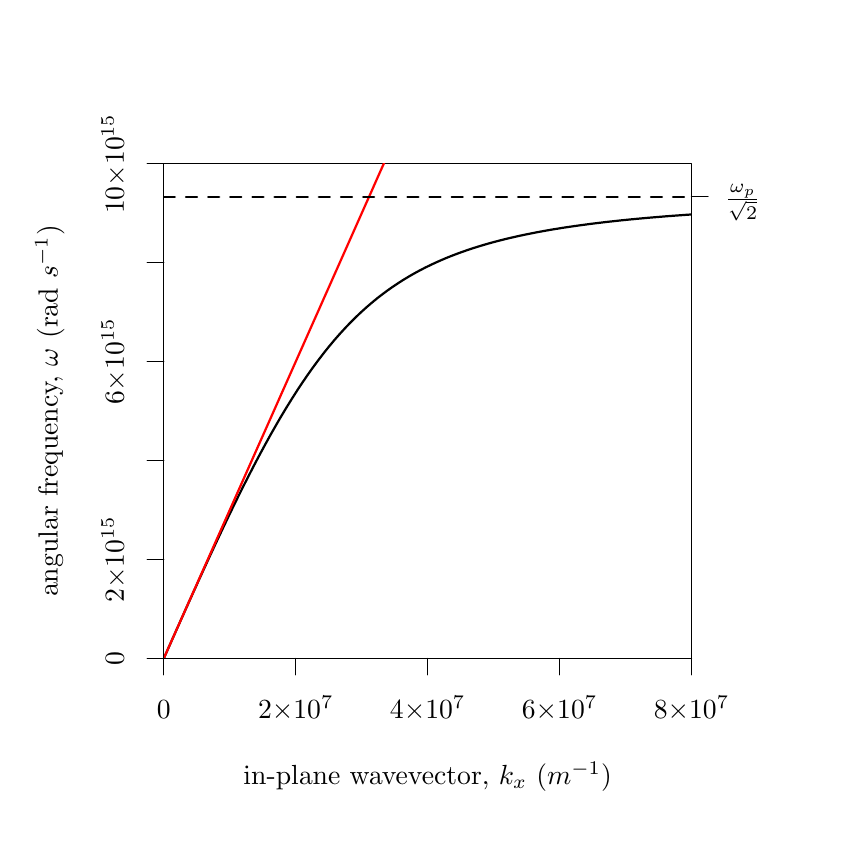
\begin{tikzpicture}[x=1pt,y=1pt]
\definecolor[named]{fillColor}{rgb}{1.00,1.00,1.00}
\path[use as bounding box,fill=fillColor,fill opacity=0.00] (0,0) rectangle (289.08,289.08);
\begin{scope}
\path[clip] (  0.00,  0.00) rectangle (289.08,289.08);
\definecolor[named]{drawColor}{rgb}{0.00,0.00,0.00}

\path[draw=drawColor,line width= 0.4pt,line join=round,line cap=round] ( 49.20, 61.20) --
	(239.88, 61.20) --
	(239.88,239.88) --
	( 49.20,239.88) --
	( 49.20, 61.20);
\end{scope}
\begin{scope}
\path[clip] (  0.00,  0.00) rectangle (289.08,289.08);
\definecolor[named]{drawColor}{rgb}{0.00,0.00,0.00}

\node[text=drawColor,anchor=base,inner sep=0pt, outer sep=0pt, scale=  1.00] at (144.54, 15.60) {in-plane wavevector, $k_x$ ($m^{-1}$)};

\node[text=drawColor,rotate= 90.00,anchor=base,inner sep=0pt, outer sep=0pt, scale=  1.00] at ( 10.80,150.54) {angular frequency, $\omega$ (rad $s^{-1}$)};
\end{scope}
\begin{scope}
\path[clip] ( 49.20, 61.20) rectangle (239.88,239.88);
\definecolor[named]{drawColor}{rgb}{0.00,0.00,0.00}

\path[draw=drawColor,line width= 0.8pt,line join=round,line cap=round] ( 49.20, 61.20) --
	( 51.13, 65.53) --
	( 53.05, 69.86) --
	( 54.98, 74.18) --
	( 56.90, 78.48) --
	( 58.83, 82.77) --
	( 60.76, 87.03) --
	( 62.68, 91.27) --
	( 64.61, 95.48) --
	( 66.53, 99.65) --
	( 68.46,103.78) --
	( 70.39,107.87) --
	( 72.31,111.90) --
	( 74.24,115.89) --
	( 76.16,119.81) --
	( 78.09,123.68) --
	( 80.02,127.47) --
	( 81.94,131.19) --
	( 83.87,134.84) --
	( 85.80,138.40) --
	( 87.72,141.89) --
	( 89.65,145.28) --
	( 91.57,148.59) --
	( 93.50,151.80) --
	( 95.43,154.91) --
	( 97.35,157.93) --
	( 99.28,160.84) --
	(101.20,163.65) --
	(103.13,166.37) --
	(105.06,168.97) --
	(106.98,171.48) --
	(108.91,173.89) --
	(110.83,176.19) --
	(112.76,178.39) --
	(114.69,180.50) --
	(116.61,182.51) --
	(118.54,184.43) --
	(120.46,186.26) --
	(122.39,188.00) --
	(124.32,189.66) --
	(126.24,191.24) --
	(128.17,192.74) --
	(130.09,194.16) --
	(132.02,195.52) --
	(133.95,196.80) --
	(135.87,198.03) --
	(137.80,199.19) --
	(139.72,200.29) --
	(141.65,201.34) --
	(143.58,202.34) --
	(145.50,203.28) --
	(147.43,204.18) --
	(149.36,205.04) --
	(151.28,205.86) --
	(153.21,206.63) --
	(155.13,207.37) --
	(157.06,208.07) --
	(158.99,208.74) --
	(160.91,209.38) --
	(162.84,209.99) --
	(164.76,210.57) --
	(166.69,211.13) --
	(168.62,211.66) --
	(170.54,212.16) --
	(172.47,212.65) --
	(174.39,213.11) --
	(176.32,213.55) --
	(178.25,213.98) --
	(180.17,214.38) --
	(182.10,214.77) --
	(184.02,215.15) --
	(185.95,215.50) --
	(187.88,215.85) --
	(189.80,216.18) --
	(191.73,216.49) --
	(193.65,216.80) --
	(195.58,217.09) --
	(197.51,217.37) --
	(199.43,217.64) --
	(201.36,217.90) --
	(203.28,218.16) --
	(205.21,218.40) --
	(207.14,218.63) --
	(209.06,218.86) --
	(210.99,219.07) --
	(212.92,219.28) --
	(214.84,219.49) --
	(216.77,219.68) --
	(218.69,219.87) --
	(220.62,220.05) --
	(222.55,220.23) --
	(224.47,220.40) --
	(226.40,220.56) --
	(228.32,220.72) --
	(230.25,220.88) --
	(232.18,221.03) --
	(234.10,221.17) --
	(236.03,221.31) --
	(237.95,221.45) --
	(239.88,221.58);
\definecolor[named]{drawColor}{rgb}{1.00,0.00,0.00}

\path[draw=drawColor,line width= 0.8pt,line join=round,line cap=round] ( 49.20, 61.20) --
	( 51.13, 65.53) --
	( 53.05, 69.86) --
	( 54.98, 74.19) --
	( 56.90, 78.53) --
	( 58.83, 82.86) --
	( 60.76, 87.19) --
	( 62.68, 91.52) --
	( 64.61, 95.85) --
	( 66.53,100.18) --
	( 68.46,104.52) --
	( 70.39,108.85) --
	( 72.31,113.18) --
	( 74.24,117.51) --
	( 76.16,121.84) --
	( 78.09,126.17) --
	( 80.02,130.51) --
	( 81.94,134.84) --
	( 83.87,139.17) --
	( 85.80,143.50) --
	( 87.72,147.83) --
	( 89.65,152.16) --
	( 91.57,156.50) --
	( 93.50,160.83) --
	( 95.43,165.16) --
	( 97.35,169.49) --
	( 99.28,173.82) --
	(101.20,178.15) --
	(103.13,182.49) --
	(105.06,186.82) --
	(106.98,191.15) --
	(108.91,195.48) --
	(110.83,199.81) --
	(112.76,204.14) --
	(114.69,208.48) --
	(116.61,212.81) --
	(118.54,217.14) --
	(120.46,221.47) --
	(122.39,225.80) --
	(124.32,230.13) --
	(126.24,234.47) --
	(128.17,238.80) --
	(130.09,243.13) --
	(132.02,247.46) --
	(133.95,251.79) --
	(135.87,256.12) --
	(137.80,260.46) --
	(139.72,264.79) --
	(141.65,269.12) --
	(143.58,273.45) --
	(145.50,277.78) --
	(147.43,282.11) --
	(149.36,286.45) --
	(150.53,289.08);
\definecolor[named]{drawColor}{rgb}{0.00,0.00,0.00}

\path[draw=drawColor,line width= 0.8pt,dash pattern=on 4pt off 4pt ,line join=round,line cap=round] ( 49.20,227.98) --
	( 51.13,227.98) --
	( 53.05,227.98) --
	( 54.98,227.98) --
	( 56.90,227.98) --
	( 58.83,227.98) --
	( 60.76,227.98) --
	( 62.68,227.98) --
	( 64.61,227.98) --
	( 66.53,227.98) --
	( 68.46,227.98) --
	( 70.39,227.98) --
	( 72.31,227.98) --
	( 74.24,227.98) --
	( 76.16,227.98) --
	( 78.09,227.98) --
	( 80.02,227.98) --
	( 81.94,227.98) --
	( 83.87,227.98) --
	( 85.80,227.98) --
	( 87.72,227.98) --
	( 89.65,227.98) --
	( 91.57,227.98) --
	( 93.50,227.98) --
	( 95.43,227.98) --
	( 97.35,227.98) --
	( 99.28,227.98) --
	(101.20,227.98) --
	(103.13,227.98) --
	(105.06,227.98) --
	(106.98,227.98) --
	(108.91,227.98) --
	(110.83,227.98) --
	(112.76,227.98) --
	(114.69,227.98) --
	(116.61,227.98) --
	(118.54,227.98) --
	(120.46,227.98) --
	(122.39,227.98) --
	(124.32,227.98) --
	(126.24,227.98) --
	(128.17,227.98) --
	(130.09,227.98) --
	(132.02,227.98) --
	(133.95,227.98) --
	(135.87,227.98) --
	(137.80,227.98) --
	(139.72,227.98) --
	(141.65,227.98) --
	(143.58,227.98) --
	(145.50,227.98) --
	(147.43,227.98) --
	(149.36,227.98) --
	(151.28,227.98) --
	(153.21,227.98) --
	(155.13,227.98) --
	(157.06,227.98) --
	(158.99,227.98) --
	(160.91,227.98) --
	(162.84,227.98) --
	(164.76,227.98) --
	(166.69,227.98) --
	(168.62,227.98) --
	(170.54,227.98) --
	(172.47,227.98) --
	(174.39,227.98) --
	(176.32,227.98) --
	(178.25,227.98) --
	(180.17,227.98) --
	(182.10,227.98) --
	(184.02,227.98) --
	(185.95,227.98) --
	(187.88,227.98) --
	(189.80,227.98) --
	(191.73,227.98) --
	(193.65,227.98) --
	(195.58,227.98) --
	(197.51,227.98) --
	(199.43,227.98) --
	(201.36,227.98) --
	(203.28,227.98) --
	(205.21,227.98) --
	(207.14,227.98) --
	(209.06,227.98) --
	(210.99,227.98) --
	(212.92,227.98) --
	(214.84,227.98) --
	(216.77,227.98) --
	(218.69,227.98) --
	(220.62,227.98) --
	(222.55,227.98) --
	(224.47,227.98) --
	(226.40,227.98) --
	(228.32,227.98) --
	(230.25,227.98) --
	(232.18,227.98) --
	(234.10,227.98) --
	(236.03,227.98) --
	(237.95,227.98) --
	(239.88,227.98);
\end{scope}
\begin{scope}
\path[clip] (  0.00,  0.00) rectangle (289.08,289.08);
\definecolor[named]{drawColor}{rgb}{0.00,0.00,0.00}

\path[draw=drawColor,line width= 0.4pt,line join=round,line cap=round] ( 49.20, 61.20) -- (239.88, 61.20);

\path[draw=drawColor,line width= 0.4pt,line join=round,line cap=round] ( 49.20, 61.20) -- ( 49.20, 55.20);

\path[draw=drawColor,line width= 0.4pt,line join=round,line cap=round] ( 96.87, 61.20) -- ( 96.87, 55.20);

\path[draw=drawColor,line width= 0.4pt,line join=round,line cap=round] (144.54, 61.20) -- (144.54, 55.20);

\path[draw=drawColor,line width= 0.4pt,line join=round,line cap=round] (192.21, 61.20) -- (192.21, 55.20);

\path[draw=drawColor,line width= 0.4pt,line join=round,line cap=round] (239.88, 61.20) -- (239.88, 55.20);

\node[text=drawColor,anchor=base,inner sep=0pt, outer sep=0pt, scale=  1.00] at ( 49.20, 39.60) {0};

\node[text=drawColor,anchor=base,inner sep=0pt, outer sep=0pt, scale=  1.00] at ( 96.87, 39.60) {2$\times 10^7$};

\node[text=drawColor,anchor=base,inner sep=0pt, outer sep=0pt, scale=  1.00] at (144.54, 39.60) {4$\times 10^7$};

\node[text=drawColor,anchor=base,inner sep=0pt, outer sep=0pt, scale=  1.00] at (192.21, 39.60) {6$\times 10^7$};

\node[text=drawColor,anchor=base,inner sep=0pt, outer sep=0pt, scale=  1.00] at (239.88, 39.60) {8$\times 10^7$};

\path[draw=drawColor,line width= 0.4pt,line join=round,line cap=round] ( 49.20, 61.20) -- ( 49.20,239.88);

\path[draw=drawColor,line width= 0.4pt,line join=round,line cap=round] ( 49.20, 61.20) -- ( 43.20, 61.20);

\path[draw=drawColor,line width= 0.4pt,line join=round,line cap=round] ( 49.20, 96.94) -- ( 43.20, 96.94);

\path[draw=drawColor,line width= 0.4pt,line join=round,line cap=round] ( 49.20,132.67) -- ( 43.20,132.67);

\path[draw=drawColor,line width= 0.4pt,line join=round,line cap=round] ( 49.20,168.41) -- ( 43.20,168.41);

\path[draw=drawColor,line width= 0.4pt,line join=round,line cap=round] ( 49.20,204.14) -- ( 43.20,204.14);

\path[draw=drawColor,line width= 0.4pt,line join=round,line cap=round] ( 49.20,239.88) -- ( 43.20,239.88);

\node[text=drawColor,rotate= 90.00,anchor=base,inner sep=0pt, outer sep=0pt, scale=  1.00] at ( 34.80, 61.20) {0};

\node[text=drawColor,rotate= 90.00,anchor=base,inner sep=0pt, outer sep=0pt, scale=  1.00] at ( 34.80, 96.94) {2$\times 10^{15}$};

\node[text=drawColor,rotate= 90.00,anchor=base,inner sep=0pt, outer sep=0pt, scale=  1.00] at ( 34.80,168.41) {6$\times 10^{15}$};

\node[text=drawColor,rotate= 90.00,anchor=base,inner sep=0pt, outer sep=0pt, scale=  1.00] at ( 34.80,239.88) {10$\times 10^{15}$};

\path[draw=drawColor,line width= 0.4pt,line join=round,line cap=round] (239.88,227.98) -- (239.88,227.98);

\path[draw=drawColor,line width= 0.4pt,line join=round,line cap=round] (239.88,227.98) -- (245.88,227.98);

\node[text=drawColor,anchor=base west,inner sep=0pt, outer sep=0pt, scale=  1.00] at (251.88,224.53) {$\frac{\omega_p}{\sqrt{2}}$};
\end{scope}
\end{tikzpicture}

\caption{\label{fig:spp-dispersion}The dispersion of a surface plasmon polariton on a planar film.}
\end{center}
\end{figure}
Figure \ref{fig:spp-dispersion} shows the dispersion of a surface plasmon polarition on a flat interface between silver and air. The dielectric function for the metal has been approximated with the Drude model. 

This dispersive curve possesses two asympotopes. As $k_x\to 0$, the dispersion approaches the light line, $\omega=ck_x$. The electric field of the surface mode at this limit has only normal components and.

Plotted on the same scale is a line representing a grazing photon along the surface, the `light-line'.  Notice that the light line and the surface plasmon polariton dispersion line do not cross. There is no solution at which the energy and momentum of free-space light is equal to that of the surface plasmon polariton. The conclusion is that free-space light incident on a metallic surface cannot resonantly drive a surface plasmon polariton. 

-from literature - sambles nash johson cristey palik
Dispersion curve
real and imaginary parts of the dispersion relation
momentum mismatch (diagrammatically)
diagram - dispersion 
diagram - cartoon of plasmon fields and ez plot
\subsection{Penetration Depth}

subsituting \ref{eq:dispersion} into \ref{eq:momentum-conservation}, we find the expression for $k_{z_m}$ is,
\begin{equation}
k_{z_m}=\pm\frac{\omega}{c} \sqrt{\varepsilon_m-\frac{\varepsilon_1\varepsilon_2}{\varepsilon_1+\varepsilon_2}}=\pm\frac{\omega}{c} \sqrt{\frac{\varepsilon_m^2}{\varepsilon_1+\varepsilon_2}}
\end{equation}
blah blah blah
\begin{equation}
k_{z_m}=\pm\frac{\omega}{c}\sqrt{\frac{\operatorname{Re}{(\varepsilon_m)}^2}{\operatorname{Re}(\varepsilon_2)}}
\end{equation}


\begin{figure}
\begin{center}
%\begin{subfigure}[]
\begin{pspicture}[](4,5) %start optics diagram (8x5) grid
	\pnode(4,2){C} %labeled nodes are the positions in the (8x5) grid
	\pnode(0.5,5){i} %labeled nodes are the positions in the (8x5) grid
	\pnode(7.5,5){r} %labeled nodes are the positions in the (8x5) grid
	\pnode(8,0.5){t}
	
	\addtopsstyle{ExtendedMirror}{hatchcolor=lightgray}
	\mirror[mirrorwidth=4,mirrortype=extended,mirrordepth=2](2,5)(2,2)(2,5)
	
\psbezier[ArrowInside=->, arrowscale=2,ArrowInsideOffset=0.01](0,2)(0,5)(2,5)(2,2)
\psbezier[ArrowInside=->, arrowscale=2,ArrowInsideOffset=0.03](0.1,2)(0.1,4)(1.9,4)(1.9,2)
\psbezier[ArrowInside=->, arrowscale=2,ArrowInsideOffset=0.03](0.2,2)(0.2,3)(1.8,3)(1.8,2)

\psbezier[ArrowInside=->, arrowscale=2,ArrowInsideOffset=0.01](4,2)(4,5)(2,5)(2,2)
\psbezier[ArrowInside=->, arrowscale=2,ArrowInsideOffset=0.03](3.9,2)(3.9,4)(2.1,4)(2.1,2)
\psbezier[ArrowInside=->, arrowscale=2,ArrowInsideOffset=0.03](3.8,2)(3.8,3)(2.2,3)(2.2,2)

\psbezier[ArrowInside=->, arrowscale=2,ArrowInsideOffset=0.03](0,2)(0,0.8)(2,0.8)(2,2)
\psbezier[ArrowInside=->, arrowscale=2,ArrowInsideOffset=0.03](0.1,2)(0.1,1.25)(1.9,1.25)(1.9,2)
\psbezier[ArrowInside=->, arrowscale=2,ArrowInsideOffset=0.03](0.2,2)(0.2,1.55)(1.8,1.55)(1.8,2)

\psbezier[ArrowInside=->, arrowscale=2,ArrowInsideOffset=0.03](4,2)(4,0.8)(2,0.8)(2,2)
\psbezier[ArrowInside=->, arrowscale=2,ArrowInsideOffset=0.03](3.9,2)(3.9,1.25)(2.1,1.25)(2.1,2)
\psbezier[ArrowInside=->, arrowscale=2,ArrowInsideOffset=0.03](3.8,2)(3.8,1.55)(2.2,1.55)(2.2,2)

\rput(0.5,0.25){$\varepsilon_2$}
\rput(0.5,4.75){$\varepsilon_1$}
\rput(2.5, 4.5){$\mathbf{E}$}
\rput[Cl](0,1.95){\red $\mathbf{+ +}$}
\rput[Cr](4,1.95){\red $\mathbf{+ +}$}
\rput(2,1.95){\blue $\mathbf{- -}$}



\end{pspicture}
%\end{subfigure}
%\begin{subfigure}[]
\begin{pspicture}[](4,5) %start optics diagram (8x5) grid
	
%	\addtopsstyle{ExtendedMirror}{hatchcolor=lightgray}
%	\mirror[mirrorwidth=4,mirrortype=extended,mirrordepth=2](2,5)(2,2)(2,5)
	
\rput(3,1.5){$\varepsilon_2$}
\rput(3,2.5){$\varepsilon_1$}
\rput(4, 2){$\lvert\mathbf{E}_z\rvert$}
\psline[linewidth=0.05]{->}(0,2)(3.5,2)
\psline[linewidth=0.05]{<->}(0,0)(0,4.75)
\psbezier[linecolor=red](0.1,4.75)(0.1,2)(3,2)(3,2)
\psbezier[linecolor=red](0.1,0)(0.1,2)(0,2)(3,2)
\rput(0,5){z}


\end{pspicture}
%\end{subfigure}
\end{center}
\caption{Imaging Scatterometer (Secondary Beam) }
\end{figure}

discuss asymptotic limits ('plasmon like' and 'photon like')
propagation length
penetration depth

\section{Surface Plasmon Polaritons excited with prism coupling}
for completeness
phase condition
-momentum state diagram (nice one drawn)
-diagram kretschmann-raether and otto
-example plot

\section{Surface plasmon polaritons on 1 dimensional gratings}
\subsection{Diffraction Gratings}
The first recorded observation of diffraction by fine structure was by peering through a silk hankacheif and oberseving rainbows. 
The coordinate system for a diffraction grating is shown in figure 1. In the `conical' mount, the plane of incident light is parallel to the grating vector, $k_{gx}$. In this orientation, the plane of incidence also contains the plane of diffraction, the plane in which diffracted orders will propagate away from the surface. The relationship between incident and diffracted light is given by the equation,
\begin{equation}
n \sin{\theta}cos{\phi} + sin{\alpha_i} = \frac{\lambda_0}{d}\label{grating-eq}
\end{equation}

Which is determined from considering the coherent interference of light from the periodic surface. 
When light impinges on a periodic surface, the surface profile constrains the wave-vector of the light to possess the same periodic character as that of the surface. The wave-vector in the plane of the surface is altered by the additon or subtraction of intergre number of grating wave-vectors, $\pm k_g$. We may rewrite equation \ref{grating-eq} in terms of the wave-vectors of the system, such that
\begin{equation}
k_0 = k_0\sin{\theta}\pm k_g
\end{equation}
As previously discussed, the wave-vector of light corresponds to the light's momentum, and so a periodic surface is shown to be able to alter the lights in-surface momentum by integer numbers of the grating's `momentum'. This provides a mechanism through which we can couple light to surface plamsons. 

\subsection{Momentum coupling by coherent scattering. }


\subsection{Surface plasmon polaritons on 2 dimensional gratings}
lattices
momentum circles 

\subsection{Coupling strength to light to SPPs on gratings}
Strength of coupling - factors
depth
shape
grating profile influencing direct scattering events

\subsection{Plasmonic band gaps}
-diagram field arrangements

\subsection{Polarization conversion}



